%\title{LaTeX Portrait Poster Template}
%%%%%%%%%%%%%%%%%%%%%%%%%%%%%%%%%%%%%%%%%
% a0poster Portrait Poster
% LaTeX Template
% Version 1.0 (22/06/13)
%
% The a0poster class was created by:
% Gerlinde Kettl and Matthias Weiser (tex@kettl.de)
% 
% Adapter by Jens Buysse for Hogeschool Gent
% This template has been downloaded from:
% http://www.LaTeXTemplates.com
%
% License:
% CC BY-NC-SA 3.0 (http://creativecommons.org/licenses/by-nc-sa/3.0/)
%
%%%%%%%%%%%%%%%%%%%%%%%%%%%%%%%%%%%%%%%%%

%----------------------------------------------------------------------------------------
%	PACKAGES AND OTHER DOCUMENT CONFIGURATIONS
%----------------------------------------------------------------------------------------

\documentclass[a0,portrait]{a0poster}

\usepackage{multicol} % This is so we can have multiple columns of text side-by-side
\columnsep=100pt % This is the amount of white space between the columns in the poster
\columnseprule=3pt % This is the thickness of the black line between the columns in the poster

\usepackage[svgnames]{xcolor} % Specify colors by their 'svgnames', for a full list of all colors available see here: http://www.latextemplates.com/svgnames-colors

\usepackage{times} % Use the times font
%\usepackage{palatino} % Uncomment to use the Palatino font

\usepackage{graphicx} % Required for including images
\graphicspath{{figures/}} % Location of the graphics files
\usepackage{booktabs} % Top and bottom rules for table
\usepackage[font=small,labelfont=bf]{caption} % Required for specifying captions to tables and figures
\usepackage{amsfonts, amsmath, amsthm, amssymb} % For math fonts, symbols and environments
\usepackage{wrapfig} % Allows wrapping text around tables and figures
\usepackage[export]{adjustbox}

\begin{document}

%----------------------------------------------------------------------------------------
%	POSTER HEADER 
%----------------------------------------------------------------------------------------

% The header is divided into two boxes:
% The first is 75% wide and houses the title, subtitle, names, university/organization and contact information
% The second is 25% wide and houses a logo for your university/organization or a photo of you
% The widths of these boxes can be easily edited to accommodate your content as you see fit

\begin{minipage}[t]{0.75\linewidth}
\VeryHuge \color{HoGentAccent1} \textbf{General Data Protection Regulation voor Software as a service met persoon\-lijke gegevensverwerking} \color{Black}\\ % Title
\Huge\textit{Een praktische analyse\\}\\[2.4cm] % Subtitle
\huge \textbf{Terryn Fréderic, Gunter Van De Velde, Lieven Smits}\\[0.5cm] % Author(s)
\huge Hogeschool Gent, Valentin Vaerwyckweg 1, 9000 Gent\\[0.4cm] % University/organization
\Large \texttt{frederic.terryn.w3919@student.hogent.be} \\
\end{minipage}
%
\begin{minipage}[t]{0.25\linewidth}

\includegraphics[width=13cm,right]{figures/HOGENT_Logo_Pos_rgb.png} 

\end{minipage}

\vspace{1cm} % A bit of extra whitespace between the header and poster content

%----------------------------------------------------------------------------------------

\begin{multicols}{2} % This is how many columns your poster will be broken into, a portrait poster is generally split into 2 columns

%----------------------------------------------------------------------------------------
%	ABSTRACT
%----------------------------------------------------------------------------------------

\color{HoGentAccent1} % Navy color for the abstract

\begin{abstract}
De GDPR is sinds 2018 van kracht als Europese regelgeving. Ondernemingen die persoonlijke gegevens opvragen, bijhouden en eventueel verwerken moeten hieraan voldoen. Voor ondernemingen die Software aanbieden als service, zijn binnen dit onderzoek maatregelen opgesteld hoe ze hun bestaande software kunnen laten voldoen aan de GDPR. \\ Er zijn algemene maatregelen opgesteld zoals sensibilisatie en 'DPIA'.  Daarnaast zijn er meer uitgelichte maatregelen zoals automatische pseudonimisatie van gegevens. En tot slot is er als uitgelichte maatregel het filteren van persoonlijke informatie uit niet-structurele data, gebruik makend van Machine Learning. 
\end{abstract}
%----------------------------------------------------------------------------------------
%	INTRODUCTION
%----------------------------------------------------------------------------------------

\color{HoGentAccent1} 
\section*{Introductie}
\color{black}
\color{black}
Sinds 2018 moeten organisaties met een vestiging in Europa, en organisaties die Europese gebruikers hebben, voldoen aan de GDPR. 

Dit is een uitgebreide set van regels opgesteld om de privacy van Europeanen te beschermen. 

Hoewel de regels eenduidig zijn, is de implementatie hiervan voor elke onderneming anders, afhankelijk van hoe persoonlijke gegevens binnen de organisatie verwerkt en bijgehouden worden.

In dit onderzoek is een poging gedaan een uitgebreide lijst van maatregelen op te stellen. Maatregelen voor ondernemingen die Software aanbieden als service, en die de bedoeling hebben ervoor te zorgen dat die bewuste software voldoet aan de eisen van de GDPR. 

Verder zijn deze maatregelen specifiek toegepast op het marktonderzoeksbureau InSites Consulting. De maatregelen die nog niet van kracht waren binnen InSites Consulting zijn uitgelicht en technisch uitgewerkt.  
%----------------------------------------------------------------------------------------
%	GEOLOGY
%----------------------------------------------------------------------------------------

\color{Black} % DarkSlateGray color for the rest of the content
\color{HoGentAccent1} 
\section*{Experimenten}
\color{black}
Als eerste stap binnen het onderzoek zijn de theoretische elementen van de GDPR die belangrijk zijn voor dit onderzoek verder uitgewerkt, en uitgelegd aan de hand van voorbeelden. 

Belangrijke elementen om te weten zijn bijvoorbeeld het recht op inzage en het recht van vergetelheid van de betrokkene. \\ Dit wil zeggen dat iemand die zijn persoonsgegevens heeft vrijgegeven op elk moment hier inzage op kan vragen, en kan vragen om die te verwijderen. 

Daarna is een onderzoek uitgevoerd welke maatregelen er kunnen en moeten getroffen worden, door ondernemingen in het algemeen, die software aanbieden. 

Er zijn meer algemene maatregelen toegelicht zoals 

\begin{itemize}
    \item Privacy Scan (Data Protection Impact Assessment)
    \item Sensibilisering en Training
    \item Contractbeheer
    \item Privacy Policy mededeling (Taal, vorm, enzoverder)
    \item Pseudo en anonimisatie van gegevens
    \item Data Security 
    \item Data Retentie
\end{itemize}

Met Data Retentie wordt bedoeld het bijhouden van informatie (op alle plaatsen) in de loop van de tijd. Volgens de GDPR mag persoonlijke data niet langer worden bijgehouden dan strikt noodzakelijk voor het bedrijf. Hiervoor zijn oplossingen gezocht en gevonden specifiek voor InSites Consulting, die persoonlijke data langer bijhield dan toegelaten was. 

\color{HoGentAccent1} 
\section*{Uitgelichte maatregelen}
\color{black}
Een specifiek probleem dat naar boven is gekomen tijdens het onderzoek is het filteren van persoonlijke data uit niet-gestructureerde data.

Een woordje uitleg: binnen de software van InSites Consulting, kan door de gebruikers op verschillende plaatsen (forum, openbare discussies) in open velden gereageerd worden. Deze open velden bevatten niet-gestructureerde data, waarin persoonlijke data kan 'verborgen' zijn. 
Wanneer een gebruiker vraagt om al zijn persoonlijke data te verwijderen, moet ook hierin gefilterd worden. 

Binnen dit onderzoek is een poging gedaan dit uit te werken door middel van Machine Learning, met Microsft Cognitive Services. 

Zowel niet-gestructureerde tekst als foto's worden door ontwikkelde applicaties automatisch gecontroleerd op persoonlijke informatie. (Op figuur 1 zie je een voorbeeld van een foto-interpretatie van Cognitive Services.)

\begin{center}\vspace{1cm}
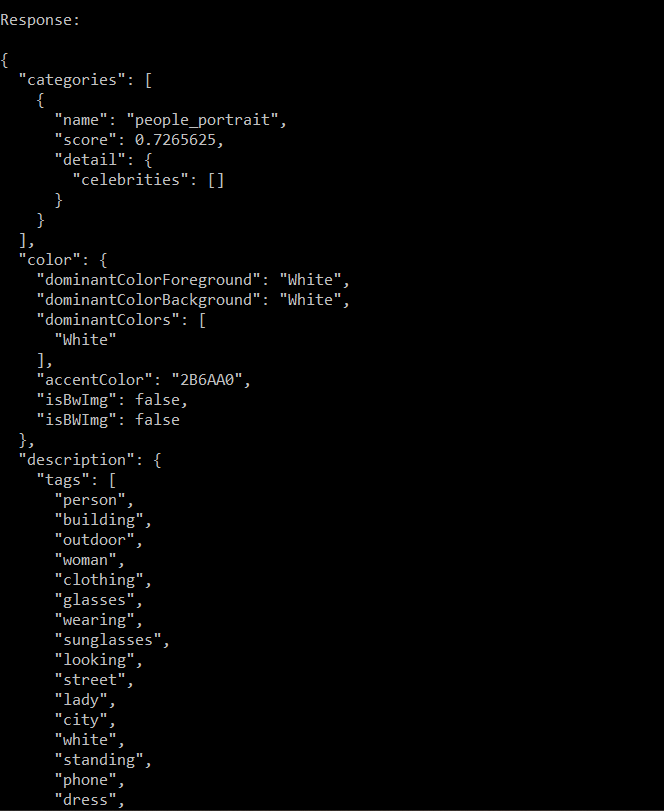
\includegraphics[width=1.0\linewidth]{JSONPICTURE}
\captionof{figure}{\color{HoGentAccent5} Het resultaat van een foto-interpratie door Microsoft Cognitive servies. Je ziet herkende categorieën en tags, die gebruikt kunnen worden om foto's met persoonlijke informatie te filteren.}
\end{center}\vspace{1cm}

%------------------------------------------------



\color{HoGentAccent1} 
\section*{Conclusies}
\color{black}
Voor elke organisatie die software aanbiedt als Service, en persoonlijke gegevens opvraagt van gebruikers, zijn vele maatregelen te treffen om aan de GDPR te voldoen. InSites Consulting heeft op heden al vele van deze maatregelen uitgevoerd, en dankzij dit onderzoek zijn de lege gaten verder opgevuld. 

De grootste uitdaging die nog rest is het volledig herkennen van persoonlijke informatie uit niet-gestructureerde tekst, aangezien Cognitive Services voorlopig enkel Engelstalige (en nog een selectie van andere talen, maar geen Nederlands), ondersteuning biedt voor textextractie. 
%----------------------------------------------------------------------------------------
%	FORTHCOMING RESEARCH
%----------------------------------------------------------------------------------------
\color{HoGentAccent1} 
\section*{Toekomstig onderzoek}
\color{black}

In de toekomst kan elke onderneming die beter wil voldoen aan de GDPR dit onderzoek als startpunt gebruiken om maatregelen te treffen en die maatregelen verder uit te diepen. Met de komst van nieuwe technologieën in de toekomst zal steeds rekening moeten gehouden worden met hoe er kan voldaan worden aan de GDPR. 

Verder is het interessant om in de toekomst op te volgen of de aangeboden Machine Learning technologieën van Microsoft ook in meerder talen beschikbaar zullen komen, zodat een beter ondersteuning kan geboden worden. 


%----------------------------------------------------------------------------------------

\end{multicols}
\end{document}